\textbf{\uline{Exemplo 06:}}
	\begin{center}
		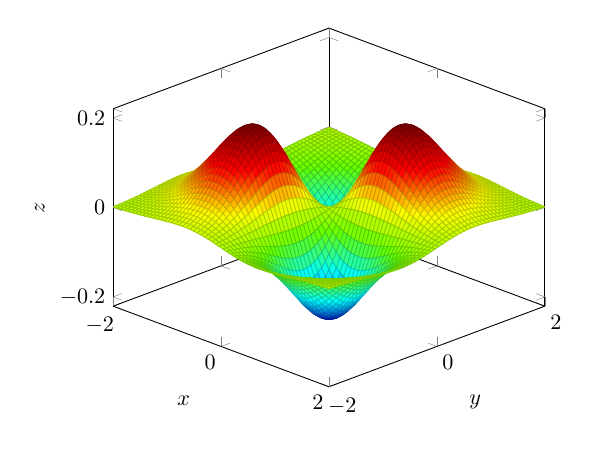
\begin{tikzpicture}[scale=0.8]
			\begin{axis}[xlabel={$x$},ylabel={$y$},zlabel={$z$},
				view={45}{30},samples=30,samples y=30]
				\addplot3[surf,
				%	shader = interp,
				samples = 60,
				samples y = 60,
				domain = -2:2,
				domain y = -2:2,
				colormap/bluered,
				]
				({x}, {y}, {x*y*exp(-x^2-y^2)});
			\end{axis}
		\end{tikzpicture}
	\end{center}